\documentclass[a4paper]{article}
\usepackage[left=1.0in,top=1.0in,right=1.0in,bottom=1.0in]{geometry}
\usepackage[english]{babel}
\usepackage[utf8]{inputenc}
\usepackage{graphicx}
\usepackage{amssymb,amsmath,amsthm,latexsym}
\graphicspath{ {./images/} }
\title{Protozoa Drawing Activity}
\author{Philip Kim}
\date{\today}
\begin{document}
\maketitle
\begin{figure}[h]
  \centering
  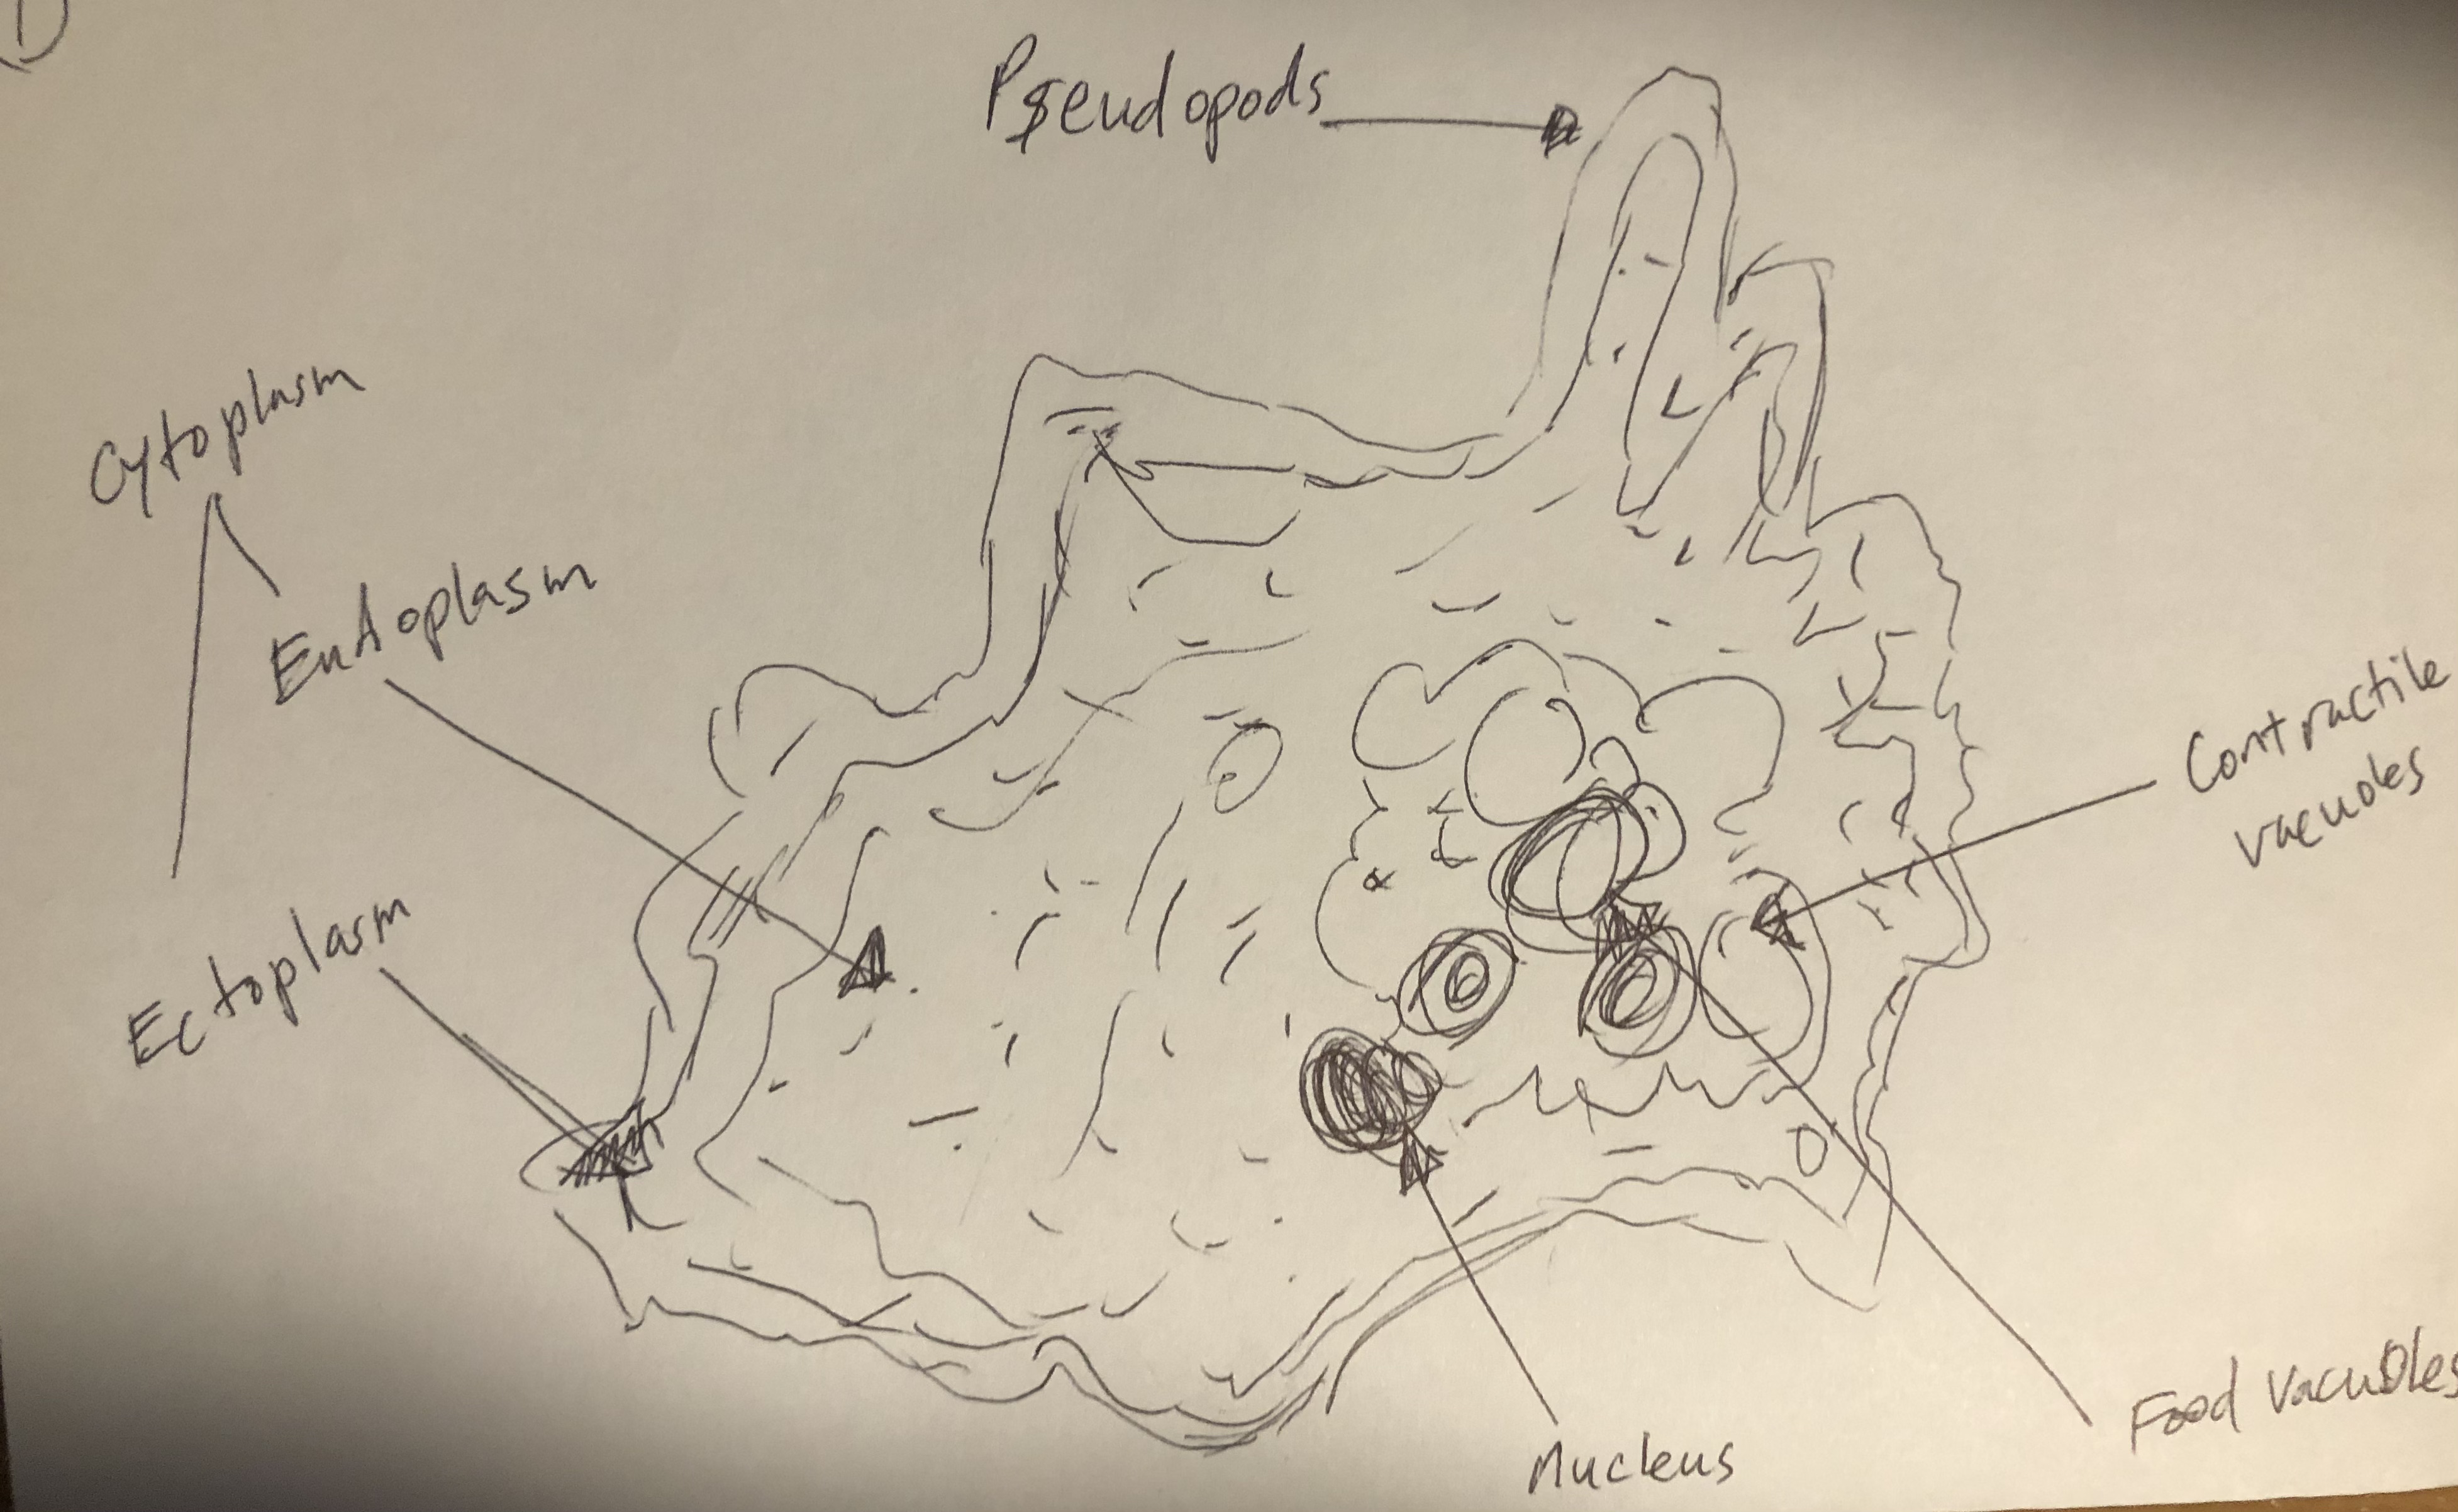
\includegraphics[width=0.5\textwidth]{amoeba.jpeg}
  \caption{\textbf{Amoeba}}
\end{figure}
\begin{enumerate}
	\item How does this organism move?
	\begin{itemize}
    \item It looks like bubbles that are controlling its movement.
  \end{itemize}
	\item What organelles are visible inside the organism and what are their functions?
	\begin{itemize}
    \item \textbf{Pseudopodia} — elongate extensions of the cell used for locomotion and feeding.
    \item \textbf{Ectoplasm} — gel-like, non-granular region of cytoplasm immediately adjacent to the cell membrane in a pseudopodium.
    \item \textbf{Endoplasm} — granular, fluid material in the central region of the cell.
    \item \textbf{Food vacuole} — a large membrane-bound chamber containing food.
    \item \textbf{Nucleus} — the dark, controlling organelle of the cell.
  \end{itemize}
	\item Based on your observations, how do you think this organism feeds?
	\begin{itemize}
    \item From observing the video, at the bottom of the amoeba it looks like the ``bubbles'' or ``circular'' objects are moving away from it and I would assume that's where they would feed through.
  \end{itemize}
\end{enumerate}
\newpage
\begin{figure}[h]
  \centering
  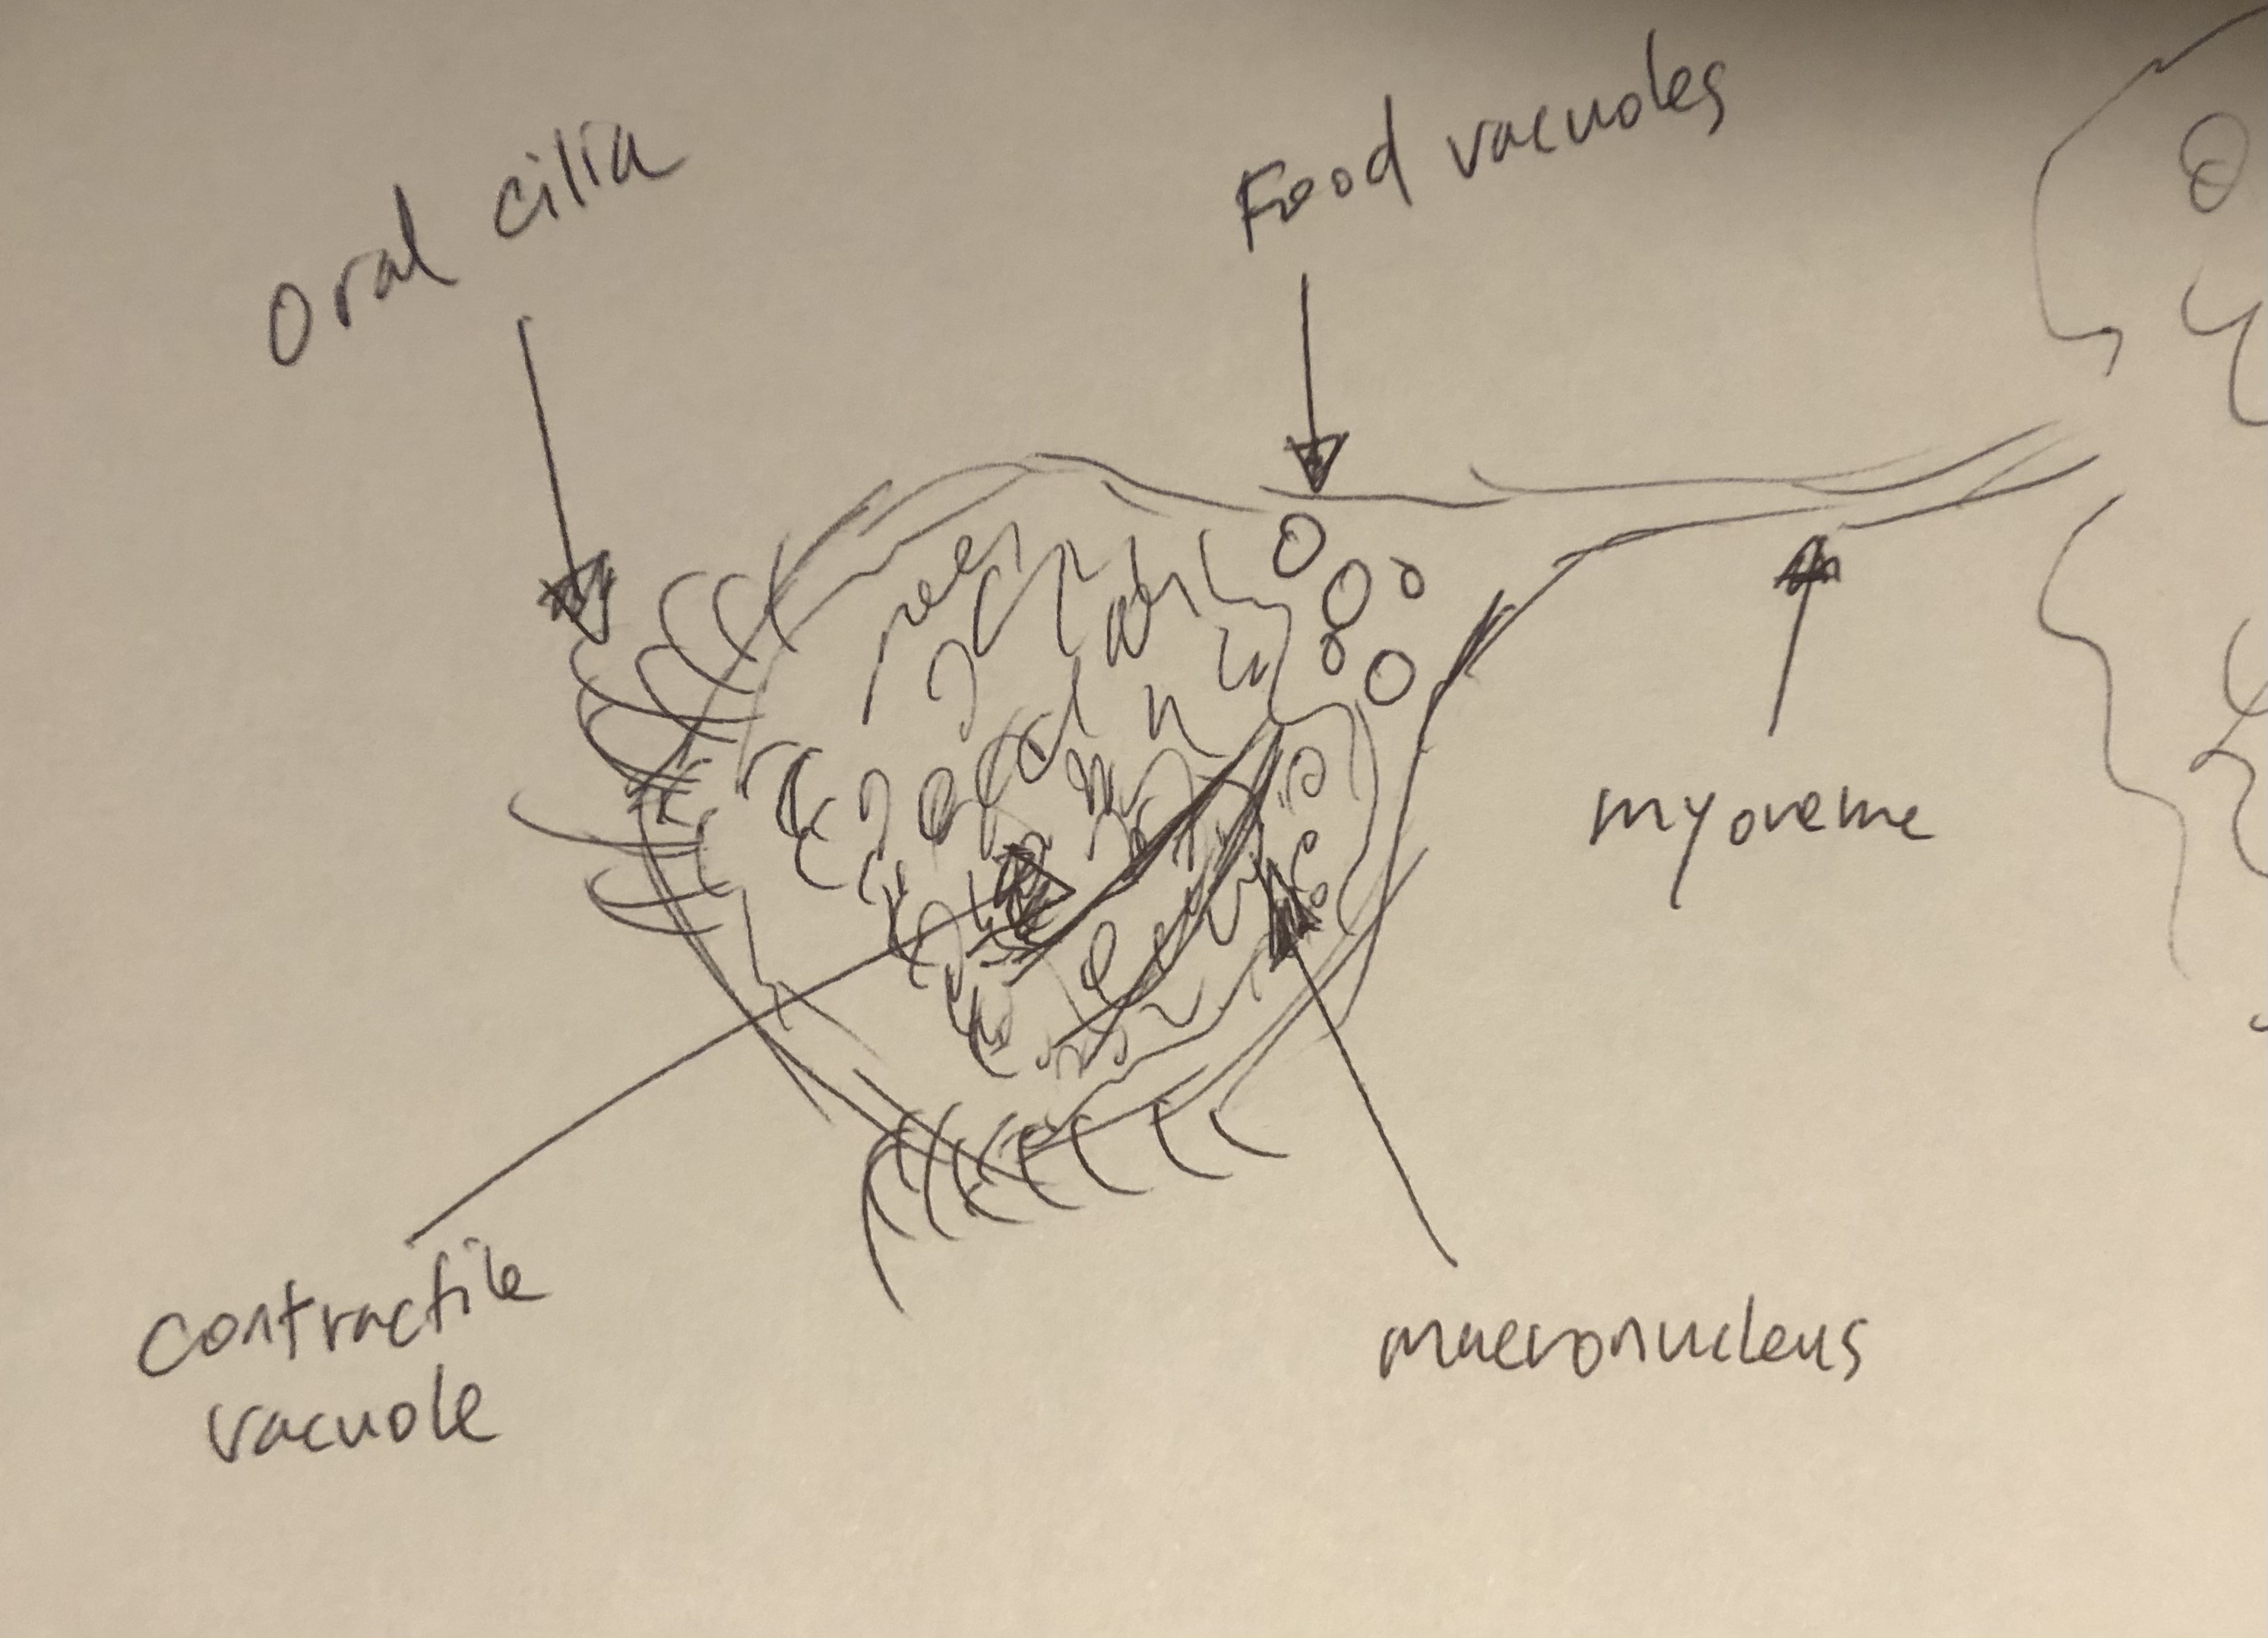
\includegraphics[width=0.5\textwidth]{vorticella.jpeg}
  \caption{\textbf{Vorticella}}
\end{figure}
\begin{enumerate}
	\item How does this organism move?
	\begin{itemize}
    \item At the tip of the vorticella, there is something that looks like eyelashes that is pulsating and possibly controlling its movement.
  \end{itemize}
	\item What organelles are visible inside the organism and what are their functions?
	\begin{itemize}
    \item \textbf{Cilia} — for scraping and filtering food.
    \item \textbf{Macronucleus} — controls cell activity.
    \item \textbf{Food vacuole} — a large membrane-bound chamber containing food.
    \item \textbf{Myoneme} consists of a series of protein filaments that shorten rapidly upon exposure to calcium.
  \end{itemize}
	\item Based on your observations, how do you think this organism feeds?
	\begin{itemize}
    \item From observing the video, at the tip it looked like it opens and closes just like a mouth would with eyelashes. I would think that it feeds through that part of it.
  \end{itemize}
\end{enumerate}
\newpage
\begin{figure}[h]
  \centering
  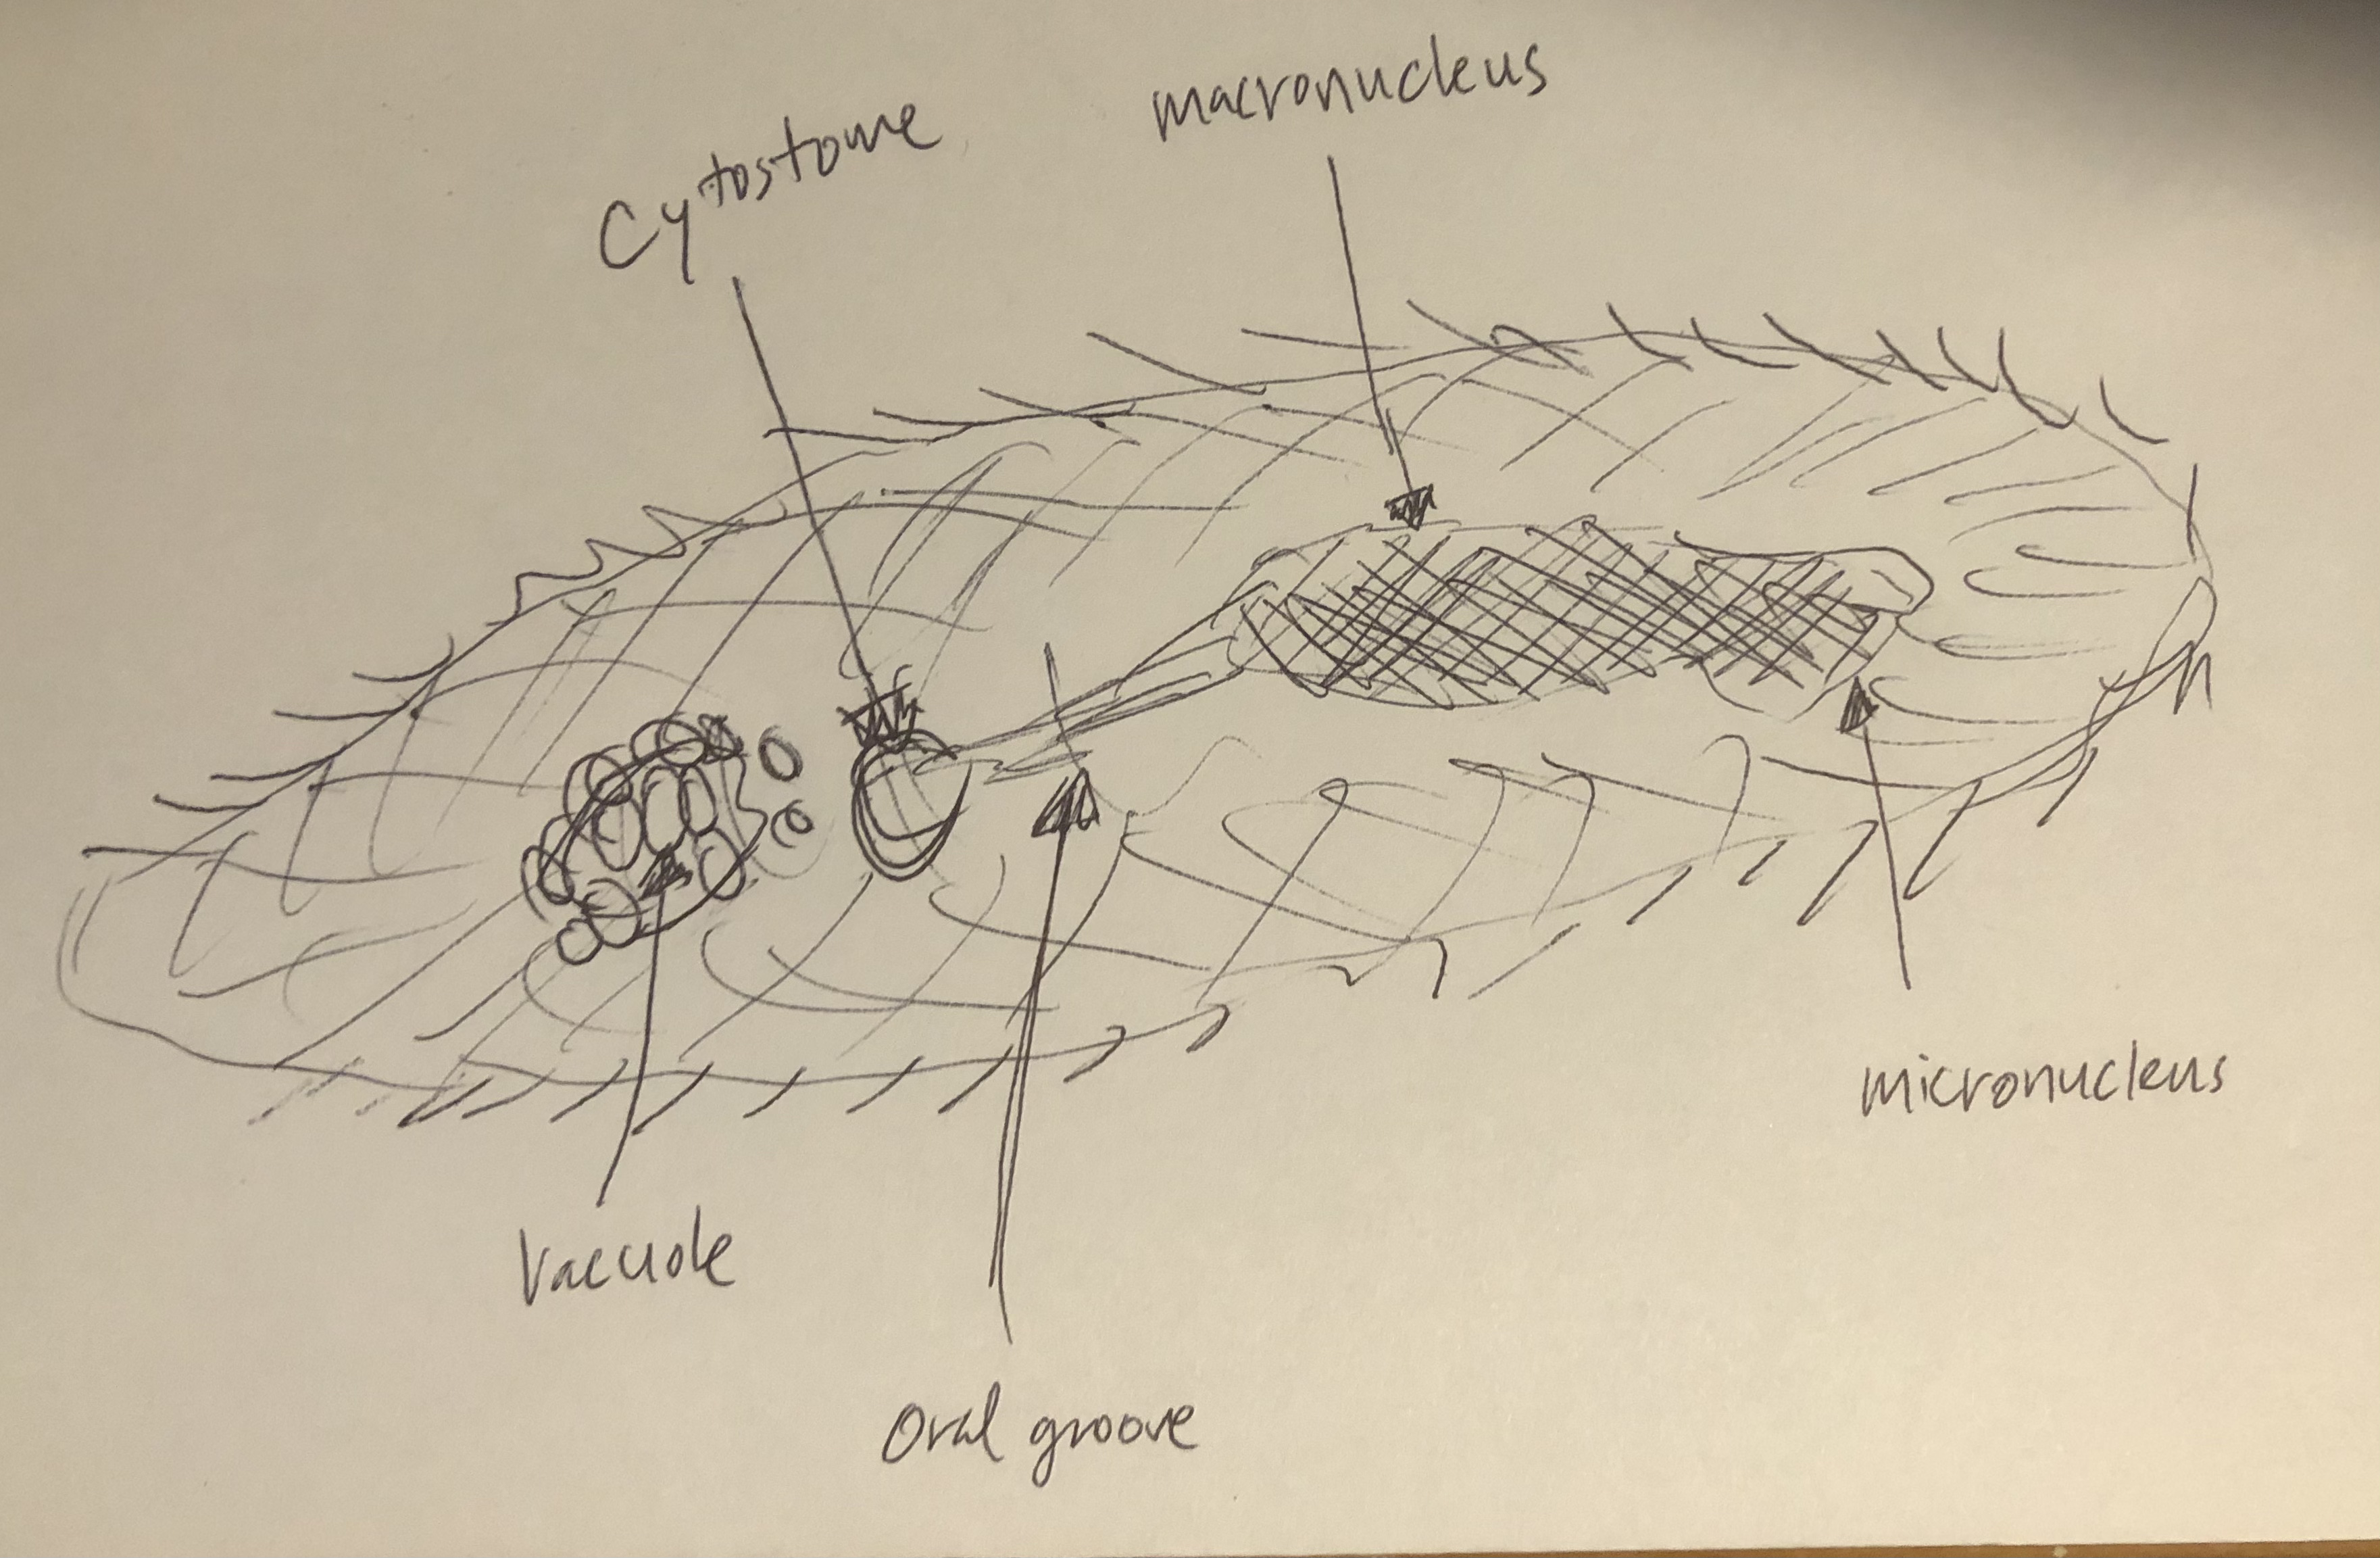
\includegraphics[width=0.5\textwidth]{paramecium.jpeg}
  \caption{\textbf{Paramecium}}
\end{figure}
\begin{enumerate}
	\item How does this organism move?
	\begin{itemize}
    \item Similar to the amoeba, it looks like the circular objects in the body is controlling its movement, but also the outer layer seems to be pulsating. Towards the end of the video a second paramecium glided through squeezing its way.
  \end{itemize}
	\item What organelles are visible inside the organism and what are their functions?
	\begin{itemize}
    \item \textbf{Micronucleus} — are exchanged during sexual reproduction.
    \item \textbf{Macronucleus} — controls cell activity.
    \item \textbf{Oral groove} — leads to the cytostome which is the mouth it feeds on.
    \item \textbf{Vacuole} — excess water accumulates in the contractile vacuoles and is discharged to the outside when the vacuoles contract.
  \end{itemize}
	\item Based on your observations, how do you think this organism feeds?
	\begin{itemize}
    \item From observing the video, this one is hard to tell because I didn't know where the front or back was until the second paramecium came into view. Even then, I still wasn't sure until I read about the oral groove which is located towards the middle that is like a stick with a ball on the end of it.
  \end{itemize}
\end{enumerate}
\newpage
\begin{figure}[h]
  \centering
  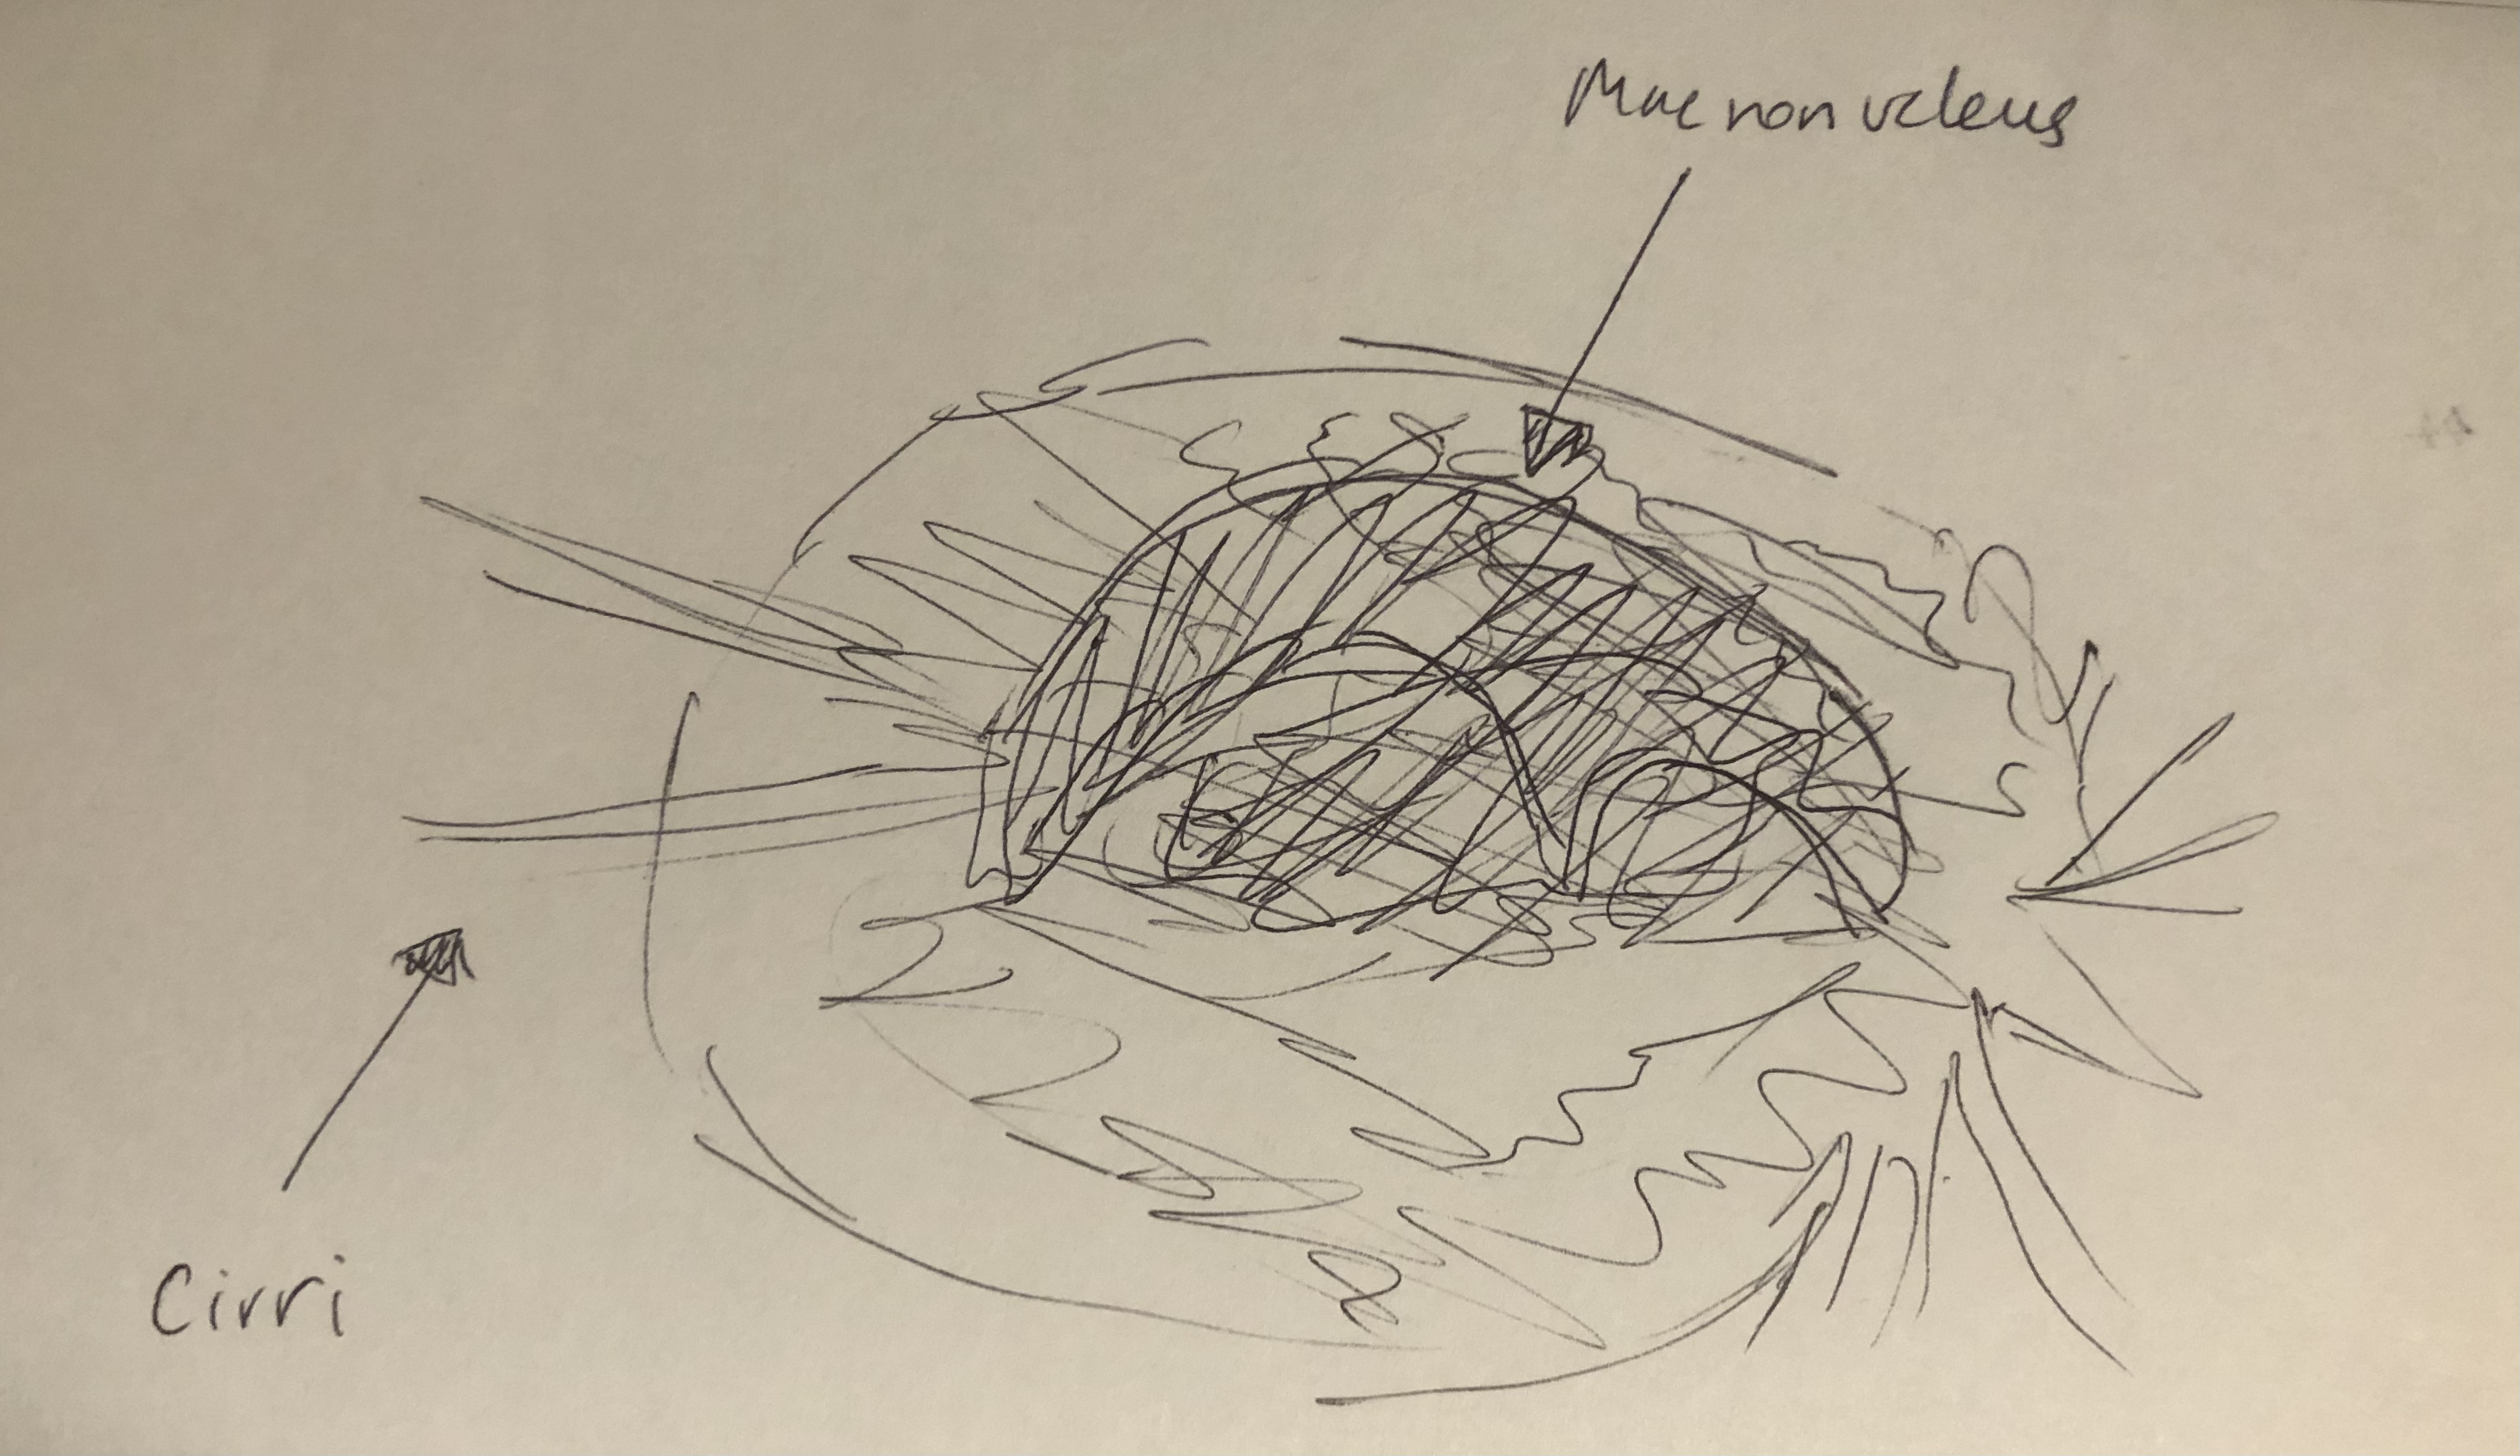
\includegraphics[width=0.5\textwidth]{euplotes.jpeg}
  \caption{\textbf{Euplotes}}
\end{figure}
\begin{enumerate}
	\item How does this organism move?
	\begin{itemize}
    \item At first it seemed like all the other protozoa with pulsating eyelash looking things, just a lot faster. But as you keep watching the video, it looks like little ticks that can fly.
  \end{itemize}
	\item What organelles are visible inside the organism and what are their functions?
	\begin{itemize}
    \item \textbf{Cirri} — helps move and feed.
    \item \textbf{Macronucleus} — typically long and narrow, and approximately horseshoe-shaped, C-shaped, or resembling the number 3, controls cell activity.
  \end{itemize}
	\item Based on your observations, how do you think this organism feeds?
	\begin{itemize}
    \item From observing the video, I would think the euplotes feed where the longer eyelashes are assuming that is the front or the face of it.
  \end{itemize}
\end{enumerate}
\end{document}
